\section{Context}

\begin{figure}[htb]
\centering
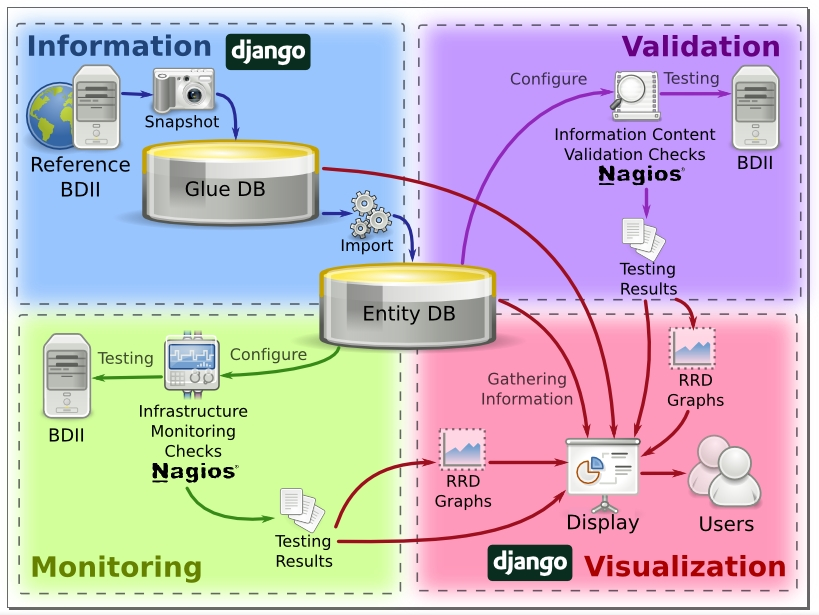
\includegraphics[width=150mm]{images/gstat-architecture.jpg}
\caption{A caption}
\label{figure:alabel}
\end{figure}

\section{Aims \& Objectives}
Different role users are going to use a portal to get information about the
performance status of the grid, to export the appropriate report for their job.
This project aims to develop these particular pieces of code to support the 
aggregation of the metrics from nagios, to allow the web based customization of
the visualization of the reports. These metrics are needed to report the
availability and reliability of NGIs and particular sites of the grid.

The procedures that are going to be used in order to achieve the above aims
should include at the beggining some opening and exploration of the environment
where the interface is going to be placed. The usage of grid computing in
the world should be well known, so a visibility of the importance and the
possible uses of the software will be recognised. The appropriate
access to the infrastructure should be gained, on different platforms and levels.
Brunel University site and GridPP/NGS VO at the beggining, as long as the UKI
ROC operations may be a good point of collaboration with researchers to reach
the bests possible requirements and data to analyse. The middleware used in
both these VOs should be examined so with the knowlege of running projects and
global usage of them may target to export better specifications. Existing
operations on the grid should also be discovered. The european initiative
milestones on the operations of the regional level should be considered as a
route, and registration to news about the upcoming research projects that
are going to use the grid should also be take place.


After that wide-opening to get the whole picture, a targeted and focused
view should follow. Existing monitoring tools must be used to check the problems
and search for requirements. The experience of SAM, Gridview, Gridmap, Gstat,
GridICE, etc should be taken in order to merge their functionality as possible
as it is. Information systems that already reside over the infrastructure, must
also be learned. Standards and specifications should be examined, on how the
message bus works and delivers the data in an hierarhical manner. A contact
with the CERN team working on MyEGEE and Indiana University's MyOSG team should
be established, to collaborate on the core of MyOSG source. Changes submission
to subversion system as long as ticket closure of the development project tool
will help to get to know the core of MyEGEE and Nagios. It is possible to create
and upstream a nagios customized web interface, to create different views of
nagios resources scheme to grid topology oriented architecture. Nagios, NRPE and
Ganglia installations should be deployed across the CE\&SE nodes of Brunel's
sites to have a working production environment to work on. Attention should be
taken on the potential performance impact of these sensors deployment. UKI
MyEGEE validation/testing portal will be used as a pre-production environment
to check changes. PNP should be fixed in GridPP Nagios to be evaluated.
Statistical access log analysis of existing tools may have results on trends of
users/admins prefered views.

Various tools are going to be used to track changes and collaborate. Monitoring
articles in GridPP wiki \& CERN twiki should be made. Snippets upstream \&
status changes must be a regular operation in SVN/JIRA/Trac in CERN interfaces.
Ongoing task through the disseration project is the reading of papers and
methodical updates of Mendeley citation management tool to have the bibliography
organized. Possible changes suggestions to MSc on DCS cource notes about grid
monitoring may by made, as long as the EGI roadmap updates. Finally with the
appropriate supervision and follow-up of meetings and presentations, a paper publishing
might take place.

\section{Organization}
\section{Literature Survey}

Grid computing \cite{li2005grid} is the most recent decade's technology
innovation in high performance computing. A large number of scientistcs working
on the operations of this huge co-operative project of EU. Monitoring \&
information architecture \cite{fisher2002datagrid} has been standardized in the
initial state of that project, to succeed in today scale of 150.000 cores. Use
of grid computing nowadays takes place in academic and research environments,
but applications in industry-based needs such as promising Power Grid control
\cite{Taylor2006} are emerging.

\subsection{Grid Monitoring}
Standards are being published about the operational models that the grid
computing initiative will use. Last decade the EGEE I, II \& III was adopted by
european universities to fund and establish a collaborative community of
researchers under a central point, the CERN oriented research project in
Particle Physics. After EGEE, the European Grid Initiative were formed to lead
to the explode of that community into regional initiatives. Performance
and availability monitoring tools and views also follow that format, phasing out
commonly used SAM \cite{egee3dsa122} and having the adoption of Nagios as the
monitoring of regional performance tool.

\subsection{Resource Brokers}
Resource Brokers \cite{Kertesz06ataxonomy} where developed to manage the
workload on Computer elements and Resource elements. Globus which is 
non-service based RB was replaced by gLite RB which is service based. A Workload
Management System (WMS) exists in gLite to do the distribution and management of
the Computing and Storage oriented tasks.

\subsection{Architecture}
A Grid Monitoring Architecture \cite{tierney2002grid} was proposed in early
2000's. Information systems were developed to create repositories of information
needed to be stored for monitoring and statistical reporting reasons. Such an
organized system later was specified by the Aggregated Topology Provider (ATP)
definition. The largest world grids adopt that model, forming OIM in OSG (USA)
and GOCDB as that information base in EGEE (Europe). Message Bus was also
defined as a mean to tranfer the undelying data, and well known tools came up
such as Gstat, GOCDB and BDII with Glue specification. Grid performance
monitoring and keeping of such an information system has also impact in the
performance of the system itshelf \cite{zhang2003performance}, so various
methods were developed to give the solution to the scalling and performance
problem, such as MDS2 (GIIS \& GRIS), GMA and R-GMA
\cite{wilson2004information}, which offers relational environment
\cite{fisher2001relational}, has experience on production systems 
\cite{byrom-production} and scales to reach huge needs such as CMS project
\cite{Bonacorsi2004,Byrom}.

\subsection{Tools}
A taxonomy effort has been made \cite{gerndt2004performance} to present the
differencies of performance monitoring systems of the grid, and later a more
general \cite{zanikolas2007importance} taxonomy paper was published to give a
more general visibility of these tools. GridICE was generaly used to aggregate
the performance metrics of ROCs in high level reports
\cite{andreozzi2005gridice}. Later GridICE was left as long as the SAM left, to
meet the milestone of EGI to have a regional monitoring tool (Nagios) to report
the reliability of the joined sites and report the values for SLA reasons.

\subsection{Sam to Nagios}
Latest EGI directive to form regional operation tools pushed the use of Nagios
\cite{imamagic2007grid} as the main tools of availability \& performance (an so
reliability) monitoring of the grid. Each NGI/ROC (regional level) has its own
interface, and hierarhicaly there is a Super Nagios interface to report the top
level view of general system availability. Nagios offers extensions such as NRPE
to remotely invoke check commands in inaccesible/private installations.
Another important add-on to Nagios is the NdoUtils, which offers an SQL store
of history data to the monitoring interface. Nagios Configuration Generator was
introduced to help the automaticaly generation of the configuration based on
the information system of nodes and services. Finally, there has been proposed
an integration of SAM views to a Nagios customized interface, to offer the last
good known SAM interface to the old users. Nagios also integrates with GGUS, a
ticketing system that european grid initiative uses.

\subsection{NGS}
Brunel Univesity takes part in regional and european initiatives. 4 different
Computer Elements exist, and 3 Storage Elements, consisting the UKI-LT2-Brunel
site. LT2 stands for London Grid, a co-operation with other London Universities.
GridPP and NGS are two collaboration groups that Brunel Univesity is member of,
and papers on the web interface \cite{Hobson2007} and real time visualization of
the grid status were presented \cite{Huang2007} by GridPP.